% BYTE Rib documentation (short).
% Build outside the repo: latexmk -pdf -outdir=<tmp> BYTE_Rib_Documentation.tex, then copy only the PDF here.
\documentclass[11pt,a4paper]{article}
\usepackage[utf8]{inputenc}
\usepackage[T1]{fontenc}
\usepackage{lmodern} % vector fonts for T1; without it MiKTeX falls back to bitmap (Type 3) fonts
\usepackage{graphicx}
\usepackage{geometry}
\usepackage{booktabs}
\usepackage{array}
\usepackage{float}
\usepackage{caption}
\usepackage{xcolor}
\usepackage{enumitem}
\usepackage{pdfpages}
\usepackage{siunitx}
\usepackage{tikz}
\usepackage[most]{tcolorbox}
\usepackage{xurl}
\usepackage[hidelinks]{hyperref}

\definecolor{customblue}{RGB}{30, 69, 114}
\definecolor{reqred}{RGB}{185, 30, 45}
\hypersetup{colorlinks=true, linkcolor=customblue, citecolor=customblue, filecolor=customblue, urlcolor=customblue}
\geometry{a4paper, margin=1in}

\newtcolorbox{reqbox}{enhanced, colback=reqred!4, colframe=reqred!80!black,
    boxrule=0.5pt, arc=2pt, left=4pt, right=4pt, top=2pt, bottom=2pt}
\newcommand{\required}[1]{\begin{reqbox}\textbf{\color{reqred}Required:} #1\end{reqbox}}
\newtcolorbox{statusbox}{enhanced, colback=customblue!5, colframe=customblue,
    boxrule=0.5pt, arc=2pt, left=4pt, right=4pt, top=2pt, bottom=2pt}
\newcommand{\net}[1]{\texttt{#1}}
\newcommand{\spinedoc}{\href{run:../../BYTE_SPIne/Documentation/BYTE_SPIne_Documentation.pdf}{SPIne documentation}}

\begin{document}

\begin{titlepage}
    \centering
    \vspace*{0.5cm}
    \includegraphics[height=11cm, page=2, trim=312 27 238 23, clip]{BYTE_Rib_Drawings.pdf}
    \vspace{1cm}

    {\Huge The ``BYTE Rib''\\[6pt] SPIne Shield \& Communication Interface\par}
    \vspace{1.5cm}
    {\normalsize 27 November 2026 \par}
    \vspace{1cm}
    {\large BYTE Rib version 1.0 (BYTE-RIB-01) \par}
    \vspace{1cm}
    {\normalsize Johnan Luca \par}
    {\normalsize BARK Project - AI Team-Robotics \par}
    \vfill
    {\footnotesize A short documentation of the BYTE Rib: purpose, pinout, protection and rules of use.
    The Rib is connected to the breakout header P3 of the BYTE SPIne, described in the \spinedoc. \par}
\end{titlepage}

\begin{statusbox}
\textbf{\color{customblue}CURRENT STATUS (27 November 2026)}

\smallskip
\begin{itemize}[leftmargin=*, nosep]
    \item \textbf{Version 1.0 ordered.} The files sent to the fab are frozen in \texttt{Releases/v1.0-ordered/}.
    \item \textbf{Not yet tested.} The bring-up checks of Section~\ref{sec:next} are still to be done.
\end{itemize}
\end{statusbox}

% ---------------------------------------------------------------------------
\section{Purpose}

The BYTE SPIne uses most of the 40-pin header of the Jetson Orin Nano. The Jetson signals that it
does not use (two I2C buses, a UART with flow control, I2S and two GPIOs) are routed one-to-one to
its $2{\times}10$ breakout header P3 (\spinedoc, section \emph{Breakout Header P3}).

The BYTE Rib turns that header into ready-to-use sensor connectors. It is connected to P3 with a
ribbon cable and provides:
\begin{itemize}[nosep]
    \item one JST PH connector per bus (two I2C, UART, I2S) carrying signals, \qty{3.3}{V} and GND;
    \item two 2-pin connectors for GPIO9 and GPIO12/PWM;
    \item ESD protection on every signal that leaves the board.
\end{itemize}

The SPIne leaves P3 unprotected on purpose and suggests placing the protection on an adapter on
the sensor side: the Rib is that adapter. The board is passive: it has no regulator, no level
translator and no pull-up resistors.

\begin{table}[H]
\centering
\begin{tabular}{ll}
\toprule
Board size & \qtyproduct{38 x 73}{mm}, corners rounded with \qty{3.5}{mm} radius \\
Layers & 2, all components on the top side \\
Components & 20 SMD/THT parts, 2 M3 mounting holes (connected to GND) \\
Supply & \net{3V3\_Jetson} from P1 pin 1 (no other rail) \\
\bottomrule
\end{tabular}
\caption{Key data.}
\end{table}

% ---------------------------------------------------------------------------
\section{Connectors and Pinout}

The input P1 (Würth 61302021821, $2{\times}10$, \qty{2.54}{mm}) has the same pinout as P3 of the
SPIne. The signal names are those of the Jetson: \net{TXD}, \net{DOUT} and \net{RTS} are Jetson
outputs, \net{RXD}, \net{DIN} and \net{CTS} are Jetson inputs.

\begin{table}[H]
\centering
\small
\setlength{\tabcolsep}{4pt}
\begin{tabular}{llll}
\toprule
Conn. & Part & Function & Pinout (pin 1 first) \\
\midrule
P1 & Würth 61302021821 & Input from SPIne P3 & see \spinedoc, table \emph{Pinout of P3} \\
J2 & JST S4B-PH-K-S & I2C1 & GND, 3V3, \net{I2C1\_SDA}, \net{I2C1\_SCL} \\
J4 & JST S4B-PH-K-S & I2C0 & GND, 3V3, \net{I2C0\_SDA}, \net{I2C0\_SCL} \\
J5 & JST S5B-PH-K-S & UART1 & GND, \net{TXD}, \net{RXD} (through R1), \net{RTS}, \net{CTS} \\
J6 & JST S6B-PH-K-S & I2S0 & GND, 3V3, \net{SCLK}, \net{FS}, \net{DIN}, \net{DOUT} \\
J1 & 691210910002 & GPIO & GND, \net{GPIO9} \\
J3 & 691210910002 & GPIO / PWM & GND, \net{GPIO12/PWM} \\
\bottomrule
\end{tabular}
\caption{Connectors of the BYTE Rib. JST PH connectors have \qty{2}{mm} pitch.}
\label{tab:conn}
\end{table}

When wiring a device, cross the UART lines: device RX to \net{TXD}, device TX to \net{RXD},
device CTS to \net{RTS} and device RTS to \net{CTS}.

% ---------------------------------------------------------------------------
\section{Protection and Passive Components}

\begin{itemize}
    \item \textbf{ESD:} four USBLC6-4SC6 low-capacitance TVS arrays (D1 UART, D2 GPIOs, D3 both I2C
    buses, D4 I2S). Their supply pin is tied to \net{3V3\_Jetson} with a \qty{100}{nF} capacitor each
    (C2, C3, C5, C6).
    Two channels of D2 are unused.
    \item \textbf{R1, \qty{1}{k\ohm}} in series with the UART receive line, between J5 pin 3 and the
    Jetson \net{UART1\_RXD}. It limits the current that an external device can inject into the Jetson
    input and into the TVS clamp, for example when the device is powered and the Jetson is not.
    \item \textbf{Decoupling:} \qty{2.2}{\micro F} next to P1 (C1) and \qty{100}{nF} at each connector
    that exports \qty{3.3}{V} (C4 on J2, C7 on J4, C8 on J6).
    \item \textbf{Test points} TP1--TP7 on the I2C, UART and GPIO12 lines, for probing without
    disconnecting the sensors.
\end{itemize}

\begin{figure}[H]
\centering
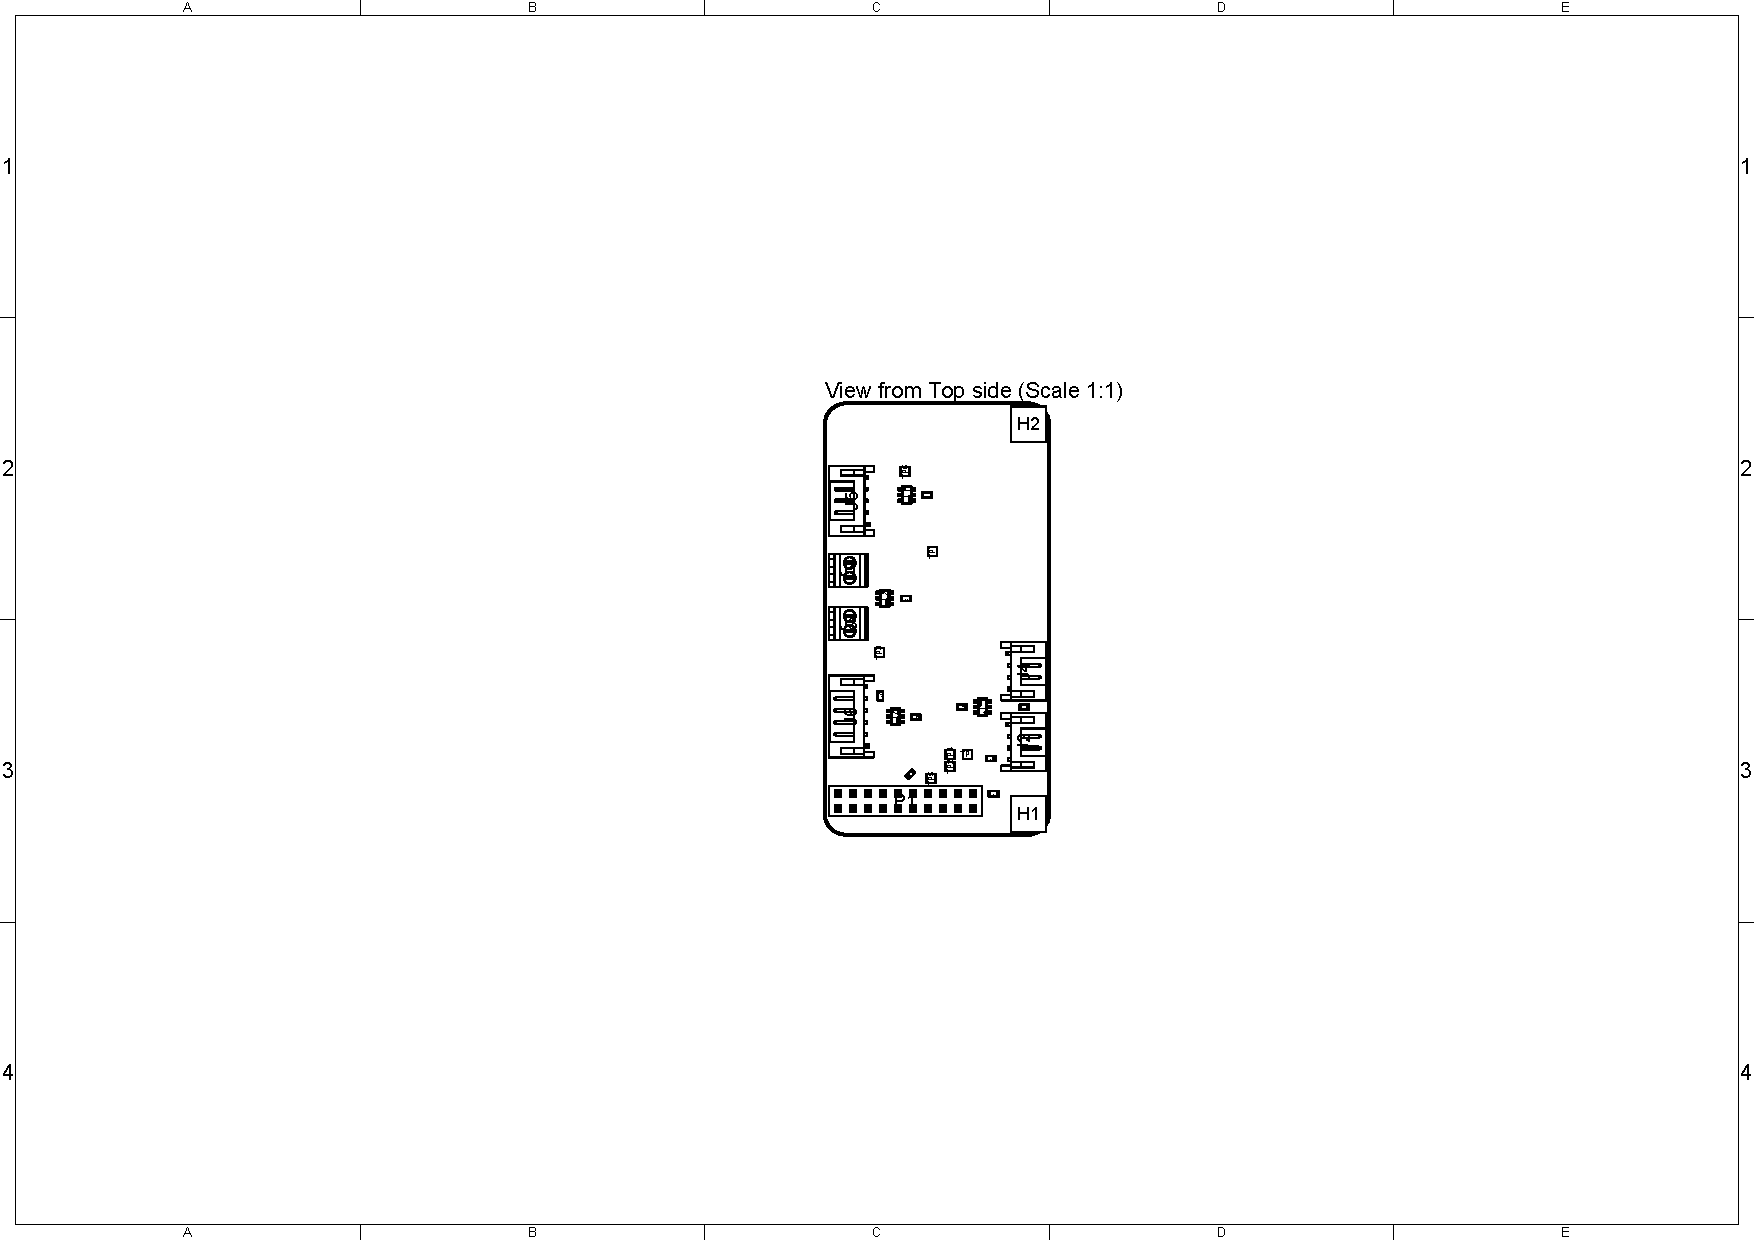
\includegraphics[height=11cm, page=1, trim=388 188 330 193, clip]{BYTE_Rib_Drawings.pdf}
\caption{Assembly drawing of the BYTE Rib, top side (Draftsman, \texttt{BYTE\_Rib.PCBDwf}).}
\end{figure}

% ---------------------------------------------------------------------------
\section{Rules of Use}

\required{the \qty{3.3}{V} on J2, J4 and J6 comes from P3 pin 1 of the SPIne and is limited to
\qty{0.1}{A} by the Jetson \textbf{in total}. Supply larger loads separately.}

\required{connect and disconnect the ribbon cable and the sensors \textbf{only with the robot switched
off}.}

\required{all signals are \qty{3.3}{V}. Do not connect \qty{5}{V} devices without a level
translator. Most header signals pass through TXB0108 translators on the Jetson carrier board, so
the constraints in the \spinedoc{} (section \emph{Level Translators on the Jetson Side}) apply,
including pull-up or pull-down resistors weaker than \qty{50}{k\ohm}.}

% ---------------------------------------------------------------------------
\section{Next Steps}\label{sec:next}

Bring-up checks, still to be done on the ordered boards:
\begin{enumerate}[nosep]
    \item visual inspection and continuity from P1 to each connector (Table~\ref{tab:conn});
    \item check that \net{3V3\_Jetson} is not shorted to GND, then power up through the SPIne;
    \item I2C scan on both buses with a sensor connected to J2 and J4;
    \item UART loopback and communication with a device on J5 at the target baud rate, including
    the receive path through R1;
    \item I2S with a microphone or amplifier on J6;
    \item GPIO9 and GPIO12/PWM on J1 and J3.
\end{enumerate}

% ---------------------------------------------------------------------------
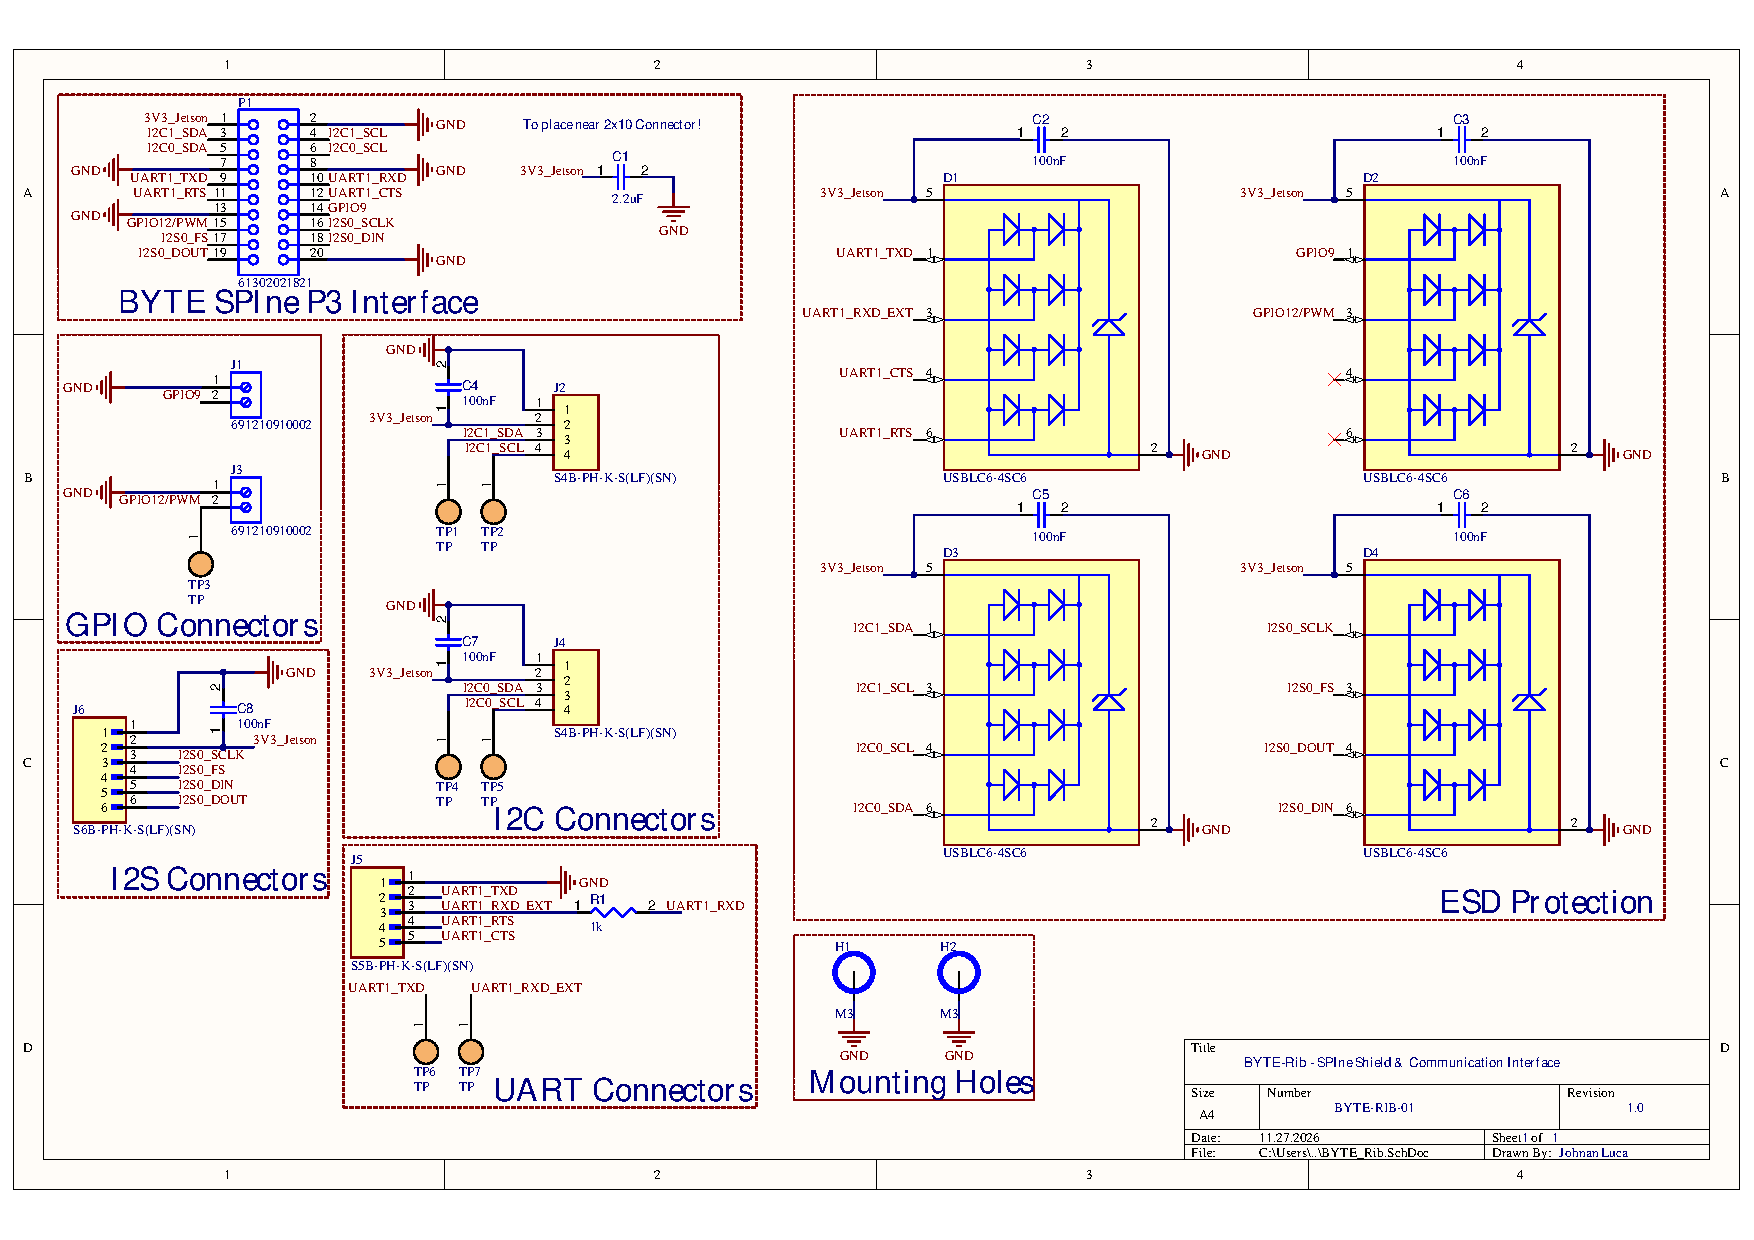
\includepdf[pages=1, fitpaper=true]{../BYTE_Rib.pdf}

\end{document}
